%\documentclass[12pt, amstex, letterpaper] {report} %{article}


\usepackage[margin=1in]{geometry}
\topmargin -0.5in \textwidth 6.5in \textheight 9in
\footskip .5in
\headheight 0.3in


\usepackage{Sweave}

\DefineVerbatimEnvironment{Sinput}{Verbatim} {xleftmargin=0em,frame=single}
\DefineVerbatimEnvironment{Soutput}{Verbatim} {xleftmargin=0em,frame=single}

\usepackage{amssymb, mathrsfs, amsmath, amsfonts}
\usepackage{enumerate, comment}
\usepackage{hyperref, natbib,apalike, float} %cite
\usepackage{color, multirow, setspace, fancyhdr,graphicx}
\usepackage{undertilde}
\usepackage[bottom]{footmisc}
\usepackage{graphicx}
\usepackage{framed}
\usepackage{subcaption}
\usepackage{amsthm}

%\doublespacing
\pagestyle{empty}
\pagestyle{fancy}
\lhead{ }
%\rhead{May 2016}
\fancyfoot{ }
\rfoot{Dissertation $|$ \thepage}
\lfoot{Chris Vanlangenberg}
\date{}

\includecomment{comment}

\newtheorem{theorem}{Theorem}[section]
\newtheorem{defn}{Definition}[section]
\newtheorem{prop}{Proposition}
\newcommand{\pro}[1]{\begin{prop}{#1}\end{prop}}

%\newtheorem{proof}{proof}
\newtheorem{rmk}{Remark}
\newcommand{\rmark}[1]{\begin{rmk}{#1}\end{rmk}}

\numberwithin{equation}{section}
\renewcommand{\footrulewidth}{0.1pt}
\renewcommand{\headrulewidth}{0.1pt}


\newcommand{\eqn}[1]{\begin{equation}{#1}\end{equation}}

\newcommand{\beq}{\begin{equation}}
\newcommand{\eeq}{\end{equation}}
%\renewcommand\refname{Literature}
\newcommand{\blue}[1]{\textcolor{blue}{\emph{#1}}}
\newcommand{\red}[1]{\textcolor{red}{\emph{#1}}}
\newcommand{\twoc}[2]{{\textcolor{blue}{#1}} and {\textcolor{red}{#2}}}


\newcommand{\xn}{x_1,\ldots, x_n}
\newcommand{\Xn}{X_1,\ldots, X_n}
\newcommand\floor[1]{\lfloor{#1}\rfloor}
\newcommand\ceil[1]{\lceil{#1}\rceil}

\newcommand{\X}{\mathcal{X}}
\newcommand{\Sp}{\mathbb{S}}
\newcommand{\R}{\mathbb{R}}
\newcommand{\C}{\mathbb{C}}
\newcommand{\pd}{positive definite }



\newcommand{\code}[1]{{\small\texttt{#1}}}
\newcommand{\pkg}[1]{{\normalfont\textsf{#1}}}
\newcommand{\var}[1] {{\normalfont\textbf{#1}}}
\newcommand{\Cm}{$C_m(\phi_P, \phi_Q)\ $}

\newcommand{\jun}{\cite{JunStein2008}}
%
%\begin{document}
%\bibliographystyle{apalike}

%%%%%%%%%%%%%%%%%%%%%%%%%%%%%%%%%%%
% Literature review
%%%%%%%%%%%%%%%%%%%%%%%%%%%%%%%%%%%

\section{Spatial Data}

What does it mean by spatial data? In general, spatial data or in other words geospatial data is information about a physical object or a measurement that can be represented by numerical values in a geographic coordinate system. Spatial data appeared to be in the form of maps in 1686 and spatial modeling did not start until 1907 (\cite{Cressie1993}). There are many questions that geoscientists and engineers are interested about spatial data. Many questions naturally arise such as how to model a spatial process and then use these models to make predictions on the process at unobserved locations. There are many challenges when modeling spatial data; every point (location observed) is a random variable and only one observation/measurement is available. However, the number of unknowns to estimate are quite large compared to the available data, which is definitely a high-dimensional problem. As an example, if data were observed at 10 locations, one is estimating the variance-covariance matrix to characterize the spatial dependency for future predictions, then there will have 55 unknown entities in the variance-covariance matrix to be estimated. We will discuss about some basic properties of geospatial data by exploring some popular data sets in the literature. \\

% \begin{figure}[H]
% \label{MSU_data_latitude}
% \centering
% 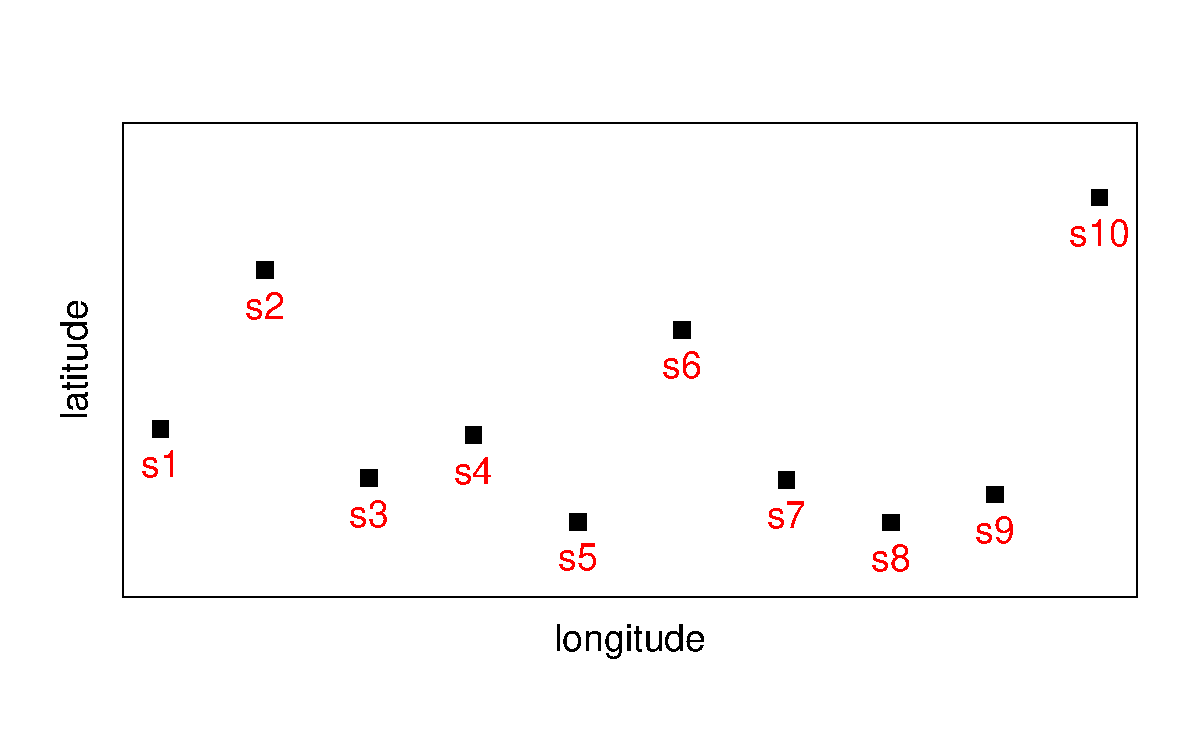
\includegraphics [width=0.8\textwidth, keepaspectratio]{graphs/location.pdf}
% \caption{Some arbitary saptial data at 10 random locations}
% \end{figure}


%\subsection{MSU data}

Since 1978 Microwave Sounding Units (MSU) measure radiation emitted by the earth's atmosphere from NOAA polar orbiting satellites. The different channels of the MSU measure different frequencies of radiation proportional to the temperature of broad vertical layers of the atmosphere. Tropospheric and lower stratospheric temperature data are collected by NOAA's TIROS-N polar-orbiting satellites and adjusted for time-dependent biases by the Global Hydrology and Climate Center at the University of Alabama in Huntsville (UAH)\footnote{\url{https://www.ncdc.noaa.gov/temp-and-precip/msu/overview}}. More information about how the data is been processed can be found in \cite{ChristySpencerBraswell2000}. Satellites do not measure temperature directly but measure radiances in various wavelength bands and then mathematically inverted to obtain the actual temperature.

% Channel 2 mainly measures tropospheric temperatures, while Channel 4 measures temperatures in the lower stratosphere. The analysis of the satellite temperature record represented here begins in 1979.

%%%%%%%%%%%%%%%%%%%%%%%%%%%%%%%%%%%%%%%%%%%%%%%%%%%%%%%%%%%%%%%%%%%%%%%%%%%%%%%%%%%%%%%%%%%%%%%%
\begin{figure}[H]
\label{MSU_data}
\centering
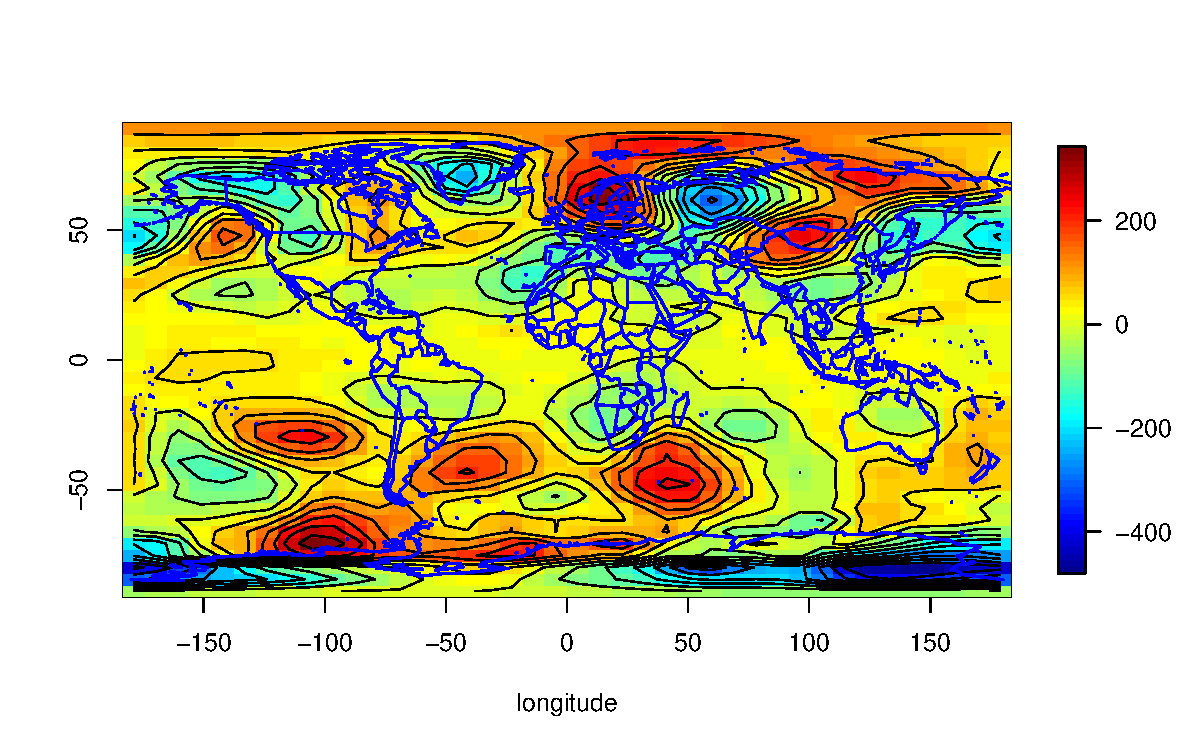
\includegraphics [width=0.8\textwidth, keepaspectratio]{graphs/MSU_data.pdf}
\caption[The MSU data were observed in August 2002 at $2.5^\circ \mbox{latitude} \times 2.5^\circ \mbox{longitude}$]{The MSU data were observed in August 2002 at $2.5^\circ \mbox{latitude} \times 2.5^\circ \mbox{longitude}$ with 10368 total number of observations.}
\end{figure}

\vfill



%%%%%%%%%%%%%%%%% below graph is not required
 % \begin{figure}[H]
 % \label{MSU_data_contour}
 % \centering
 % 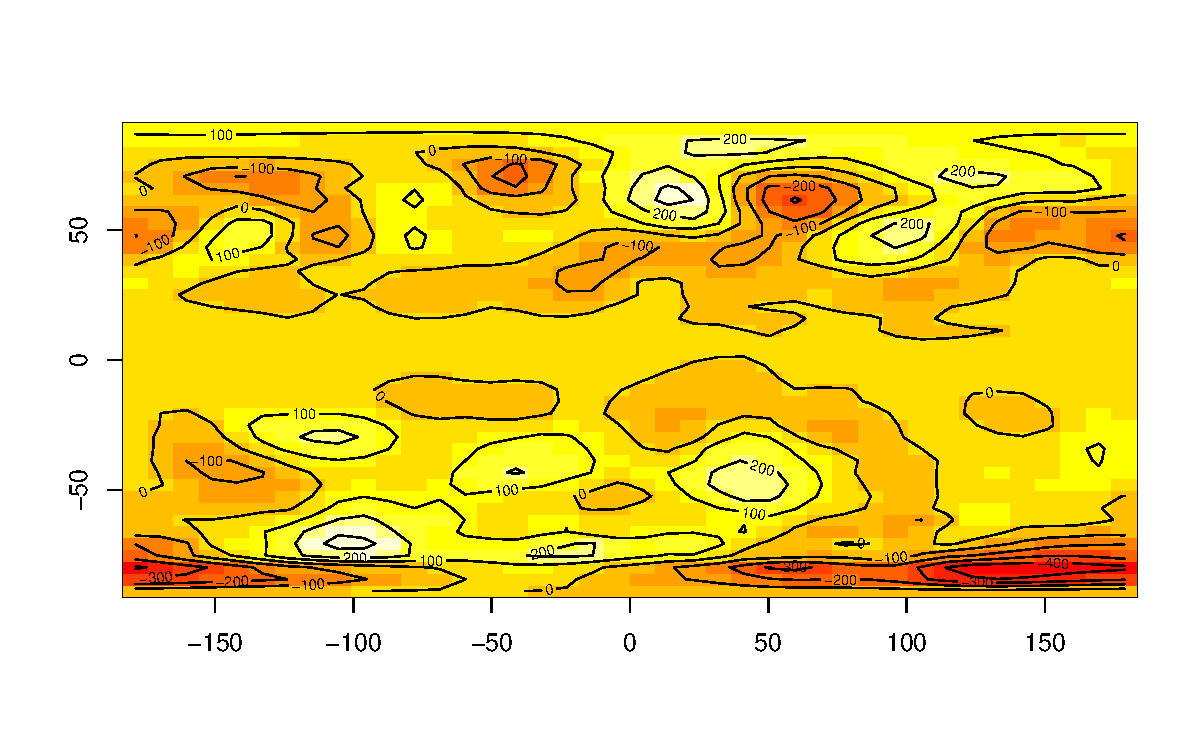
\includegraphics [height=4in, keepaspectratio]{MSU_data_contour.pdf}
 % \caption{August 2002, MSU data contour plot : resolution $2.5^0 latitude \times 2.5^0 longitude$}
 % \end{figure}


%%%%%%%%%%%%%%%%%%%%%%%%%%%%%%%%%%%%%%%%%%%%%%%%%%%%%%%%%%%%%%%%%%%%%%%%%%%%%%%%
\begin{figure}[H]
	\begin{subfigure}{.5\textwidth}
		\centering
		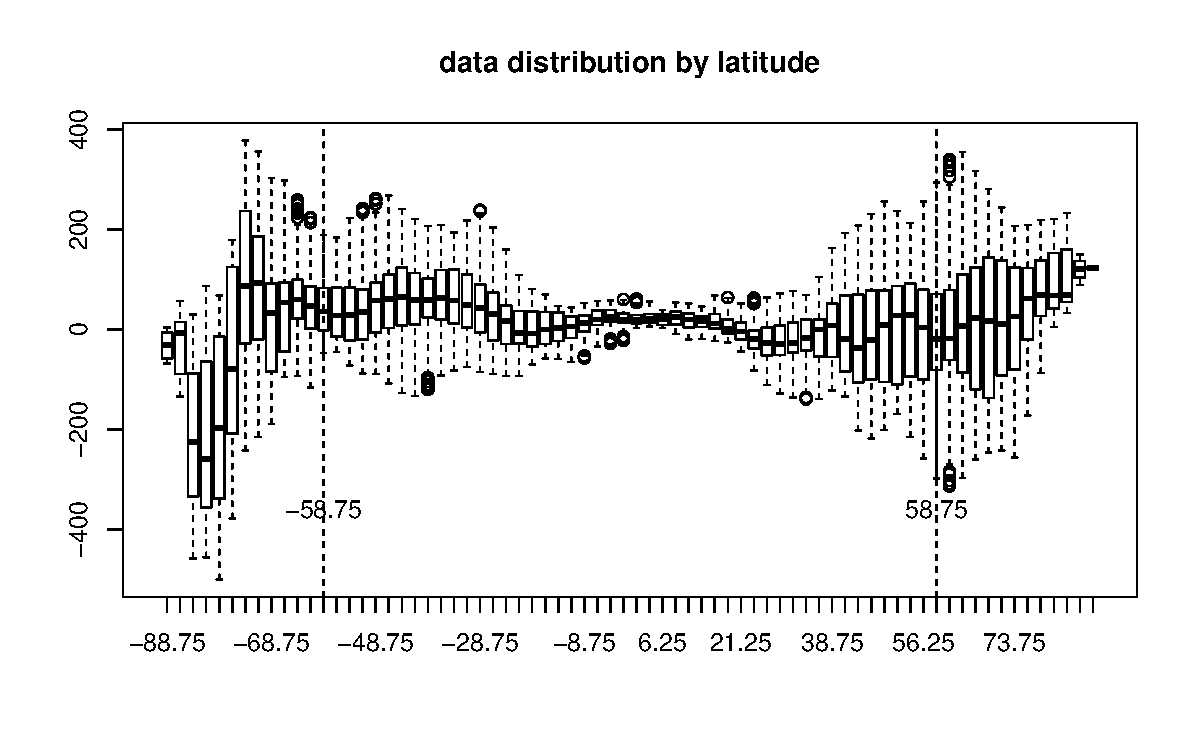
\includegraphics[width=1\linewidth]{graphs//MSU_data_latitude}
		\caption{distribution at each latitude}
		\label{MSU_data_latitude}
	\end{subfigure}
	\begin{subfigure}{.5\textwidth}
		\centering
		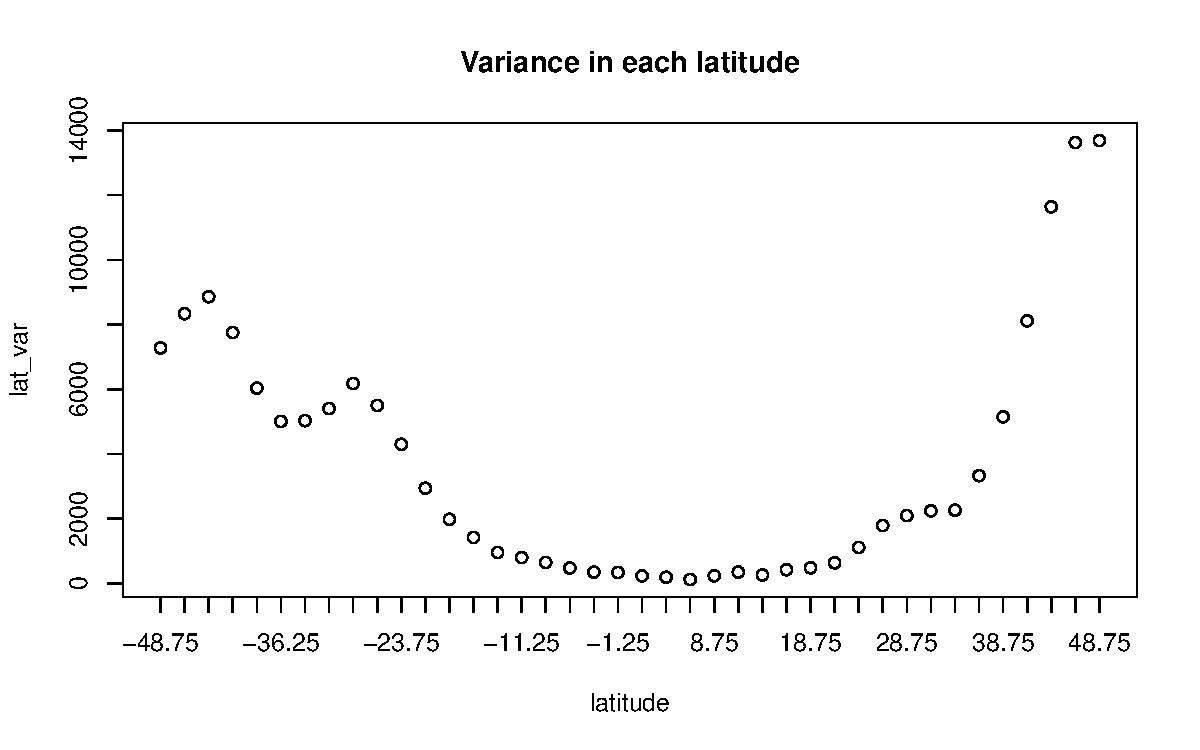
\includegraphics[width=1\linewidth]{graphs/MSU_data_var_lat}
		\caption{variance at each latitude}
		\label{MSU_data_var_lat}
	\end{subfigure}
	\caption[MSU data distribution at each latitude (data between $60^\circ S$ and $60^\circ N$]{MSU data distribution at each latitude (data between $60^\circ S$ and $60^\circ N$ were considered)}
	\label{compare_varigram_sim_2}
\end{figure}


Level 3 Total Ozone Mapping Spectrometer (TOMS) data \footnote{\url{http://disc.sci.gsfc.nasa.gov/data/datapool/TOMS}} is another popluar global data set discussed literature which has more than 20000 sapatial points (gridded points) (\cite{Stein2007}, \cite{CressieJohannesson2008}, \cite{JunStein2008}). There were some missing values in this data set. \cite{Stein2007} used the average of 8 neighboring locations to replace the missing values. They used spherical harmonics with associated Legendre polynomials of up to 78 covariates to remove the spatial trends to study axially symmetry (discussed in chapter 4) of the global data.

\vfill

% Extracted from \cite{Stein2007} ``The Nimbus-7 satellite carried a Total Ozone Mapping Spectrometer (TOMS) instrument that measured total column ozone daily from November 1, 1978 to May 6, 1993. This satellite followed a Sun-synchronous polar orbit with an orbital frequency of 13.825 orbits a day (cycle time about 104 minutes). As the satellite orbited, a scanning mirror repeatedly scanned across a track about 3000 km wide, each track yielding 35 total column ozone measurements. This version of the data is known as Level 2 and is . "

%%%%%%%%%%%%%%%%%%%%%%%%%%%%%%%%%%%%%%%%%%%%%%%%%%%%%%%%%%%%%%%%%%%%%%%%%%%%%%%%%%%%%%%%%%%%%%%%%%%%%%%
\begin{figure}[H]
\label{TOMS_data}
\centering
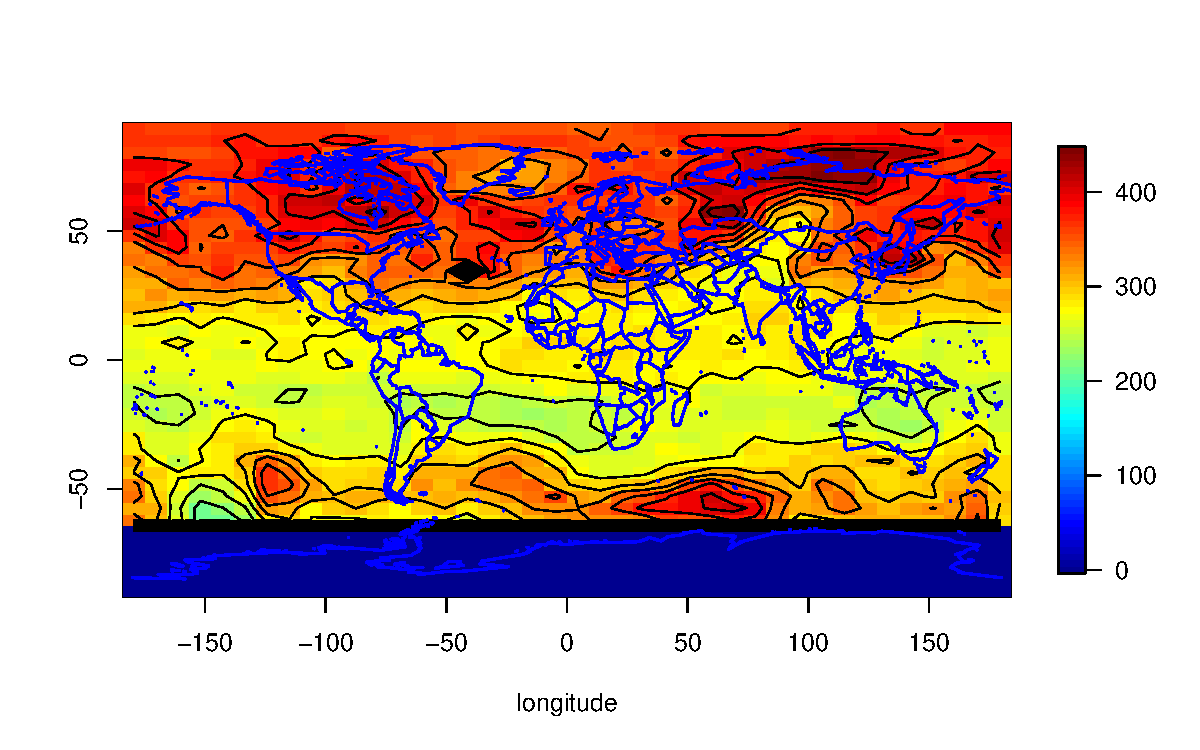
\includegraphics [width=0.8\textwidth, keepaspectratio]{graphs/TOMS_data.pdf}
\caption [TOMS data: resolution $1^\circ \mbox{latitude } \times 1.25^\circ \mbox{ longitude}$ in May, 1-6 1990.]{TOMS data: resolution $1^\circ \mbox{latitude } \times 1.25^\circ \mbox{ longitude}$ in May, 1-6 1990. The instrument used backscattered sunlight, therefore measurements were not available south of $73^\circ S$ during this week.}
\end{figure}

%%%%%%%%%%%%%%%%%%%%%%%%%%%%%%%%%%%%%%%%%%%%%%%%%%%%%%%%%%%%%%%%%%%%%%%%%%%%%%%%%%%%%%%%%%%%%%%%%%%%%%%%
\begin{figure}[H]
	\begin{subfigure}{.5\textwidth}
		\centering
		\includegraphics[width=1\linewidth]{graphs//TOMS_data_latitude}
		\caption{distribution at each latitude}
		\label{TOMS_data_latitude}
	\end{subfigure}
	\begin{subfigure}{.5\textwidth}
		\centering
		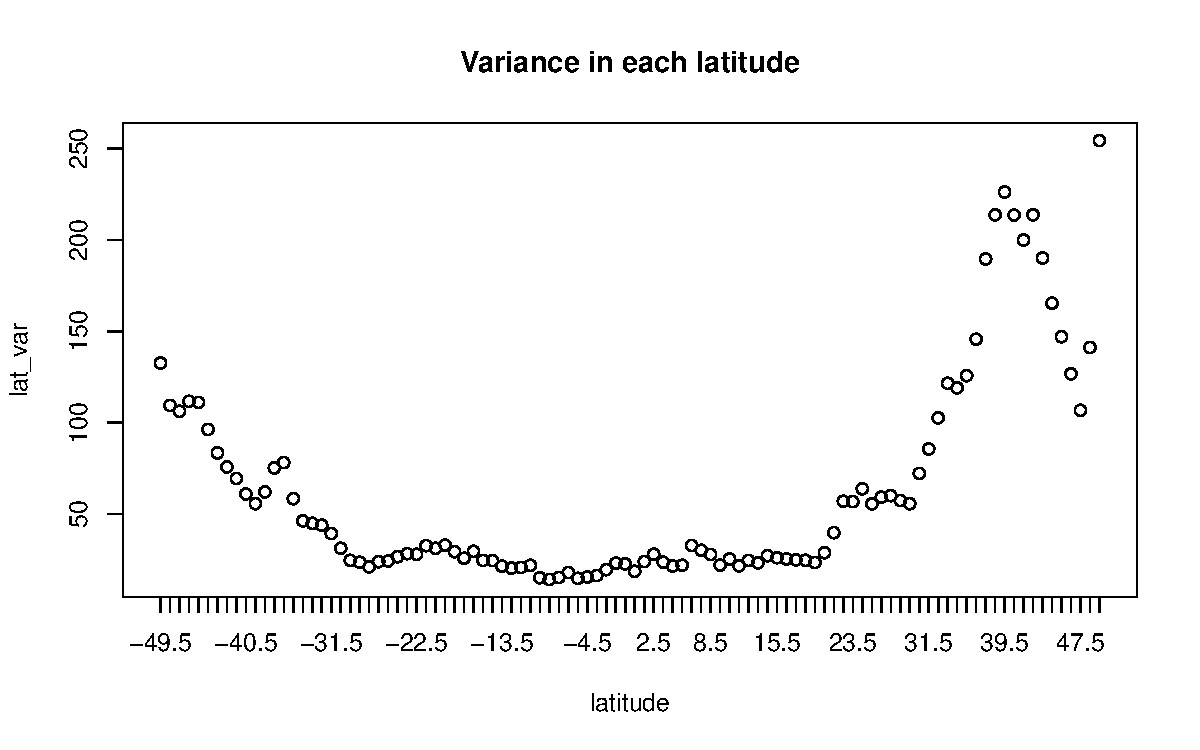
\includegraphics[width=1\linewidth]{graphs/TOMS_data_var_lat}
		\caption{variance at each latitude}
		\label{TOMS_data_var_lat}
	\end{subfigure}
	\caption[TOMS data distribution at each latitude (data between $50^\circ S$ and $50^\circ N$]{TOMS data distribution at each latitude (data between $50^\circ S$ and $50^\circ N$ were considered)}
	\label{compare_varigram_sim_2}
\end{figure}


Both MSU and TOMS data demonstrate strong variation when it is closer to Earth's poles. This shows the complexity of geospatial data. In addition, collecting geospatial data could be very expensive and time consuming. Next we discuss about the challenges when modeling spatial data.


 % \begin{figure}[H]
 % \centering
 % \includegraphics [width=0.8\textwidth, keepaspectratio]{graphs/TOMS_data_latitude.pdf}
 % \caption[OMS data: data distribution at each latitude (data between $50^\circ S$]{TOMS data: data distribution at each latitude (data between $50^\circ S$ and $50^\circ N$ were considered)}
 % \label{TOMS_data_latitude}
 % \end{figure}
 % 
 % \begin{figure}[H]
 % \centering
 % 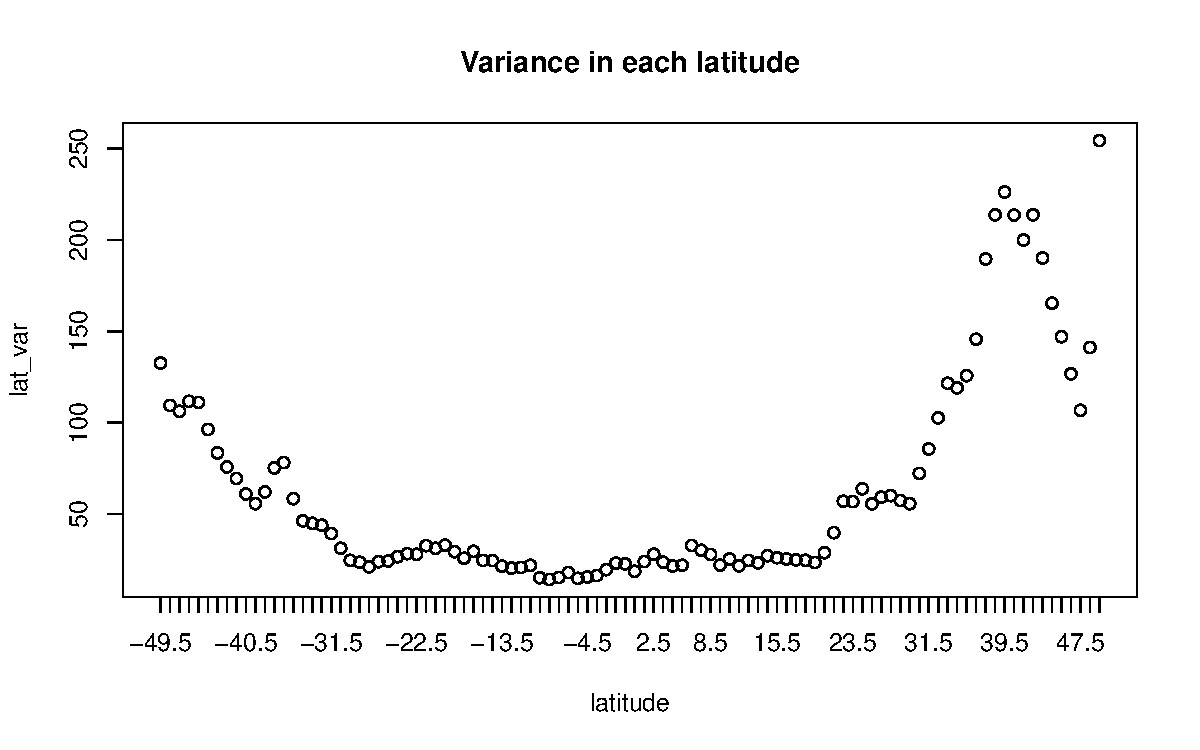
\includegraphics [width=0.8\textwidth, keepaspectratio]{graphs/TOMS_data_var_lat.pdf}
 % \caption{TOMS data: between $50^\circ S$ and $50^\circ N$, the variance at each latitude (variance is almost zero near the equator)}
 % \label{TOMS_data_var_lat}
 % \end{figure}

% \subsection{Challenges}



\section{Literature review}

There have been extensive statistical research on methodologies and techniques developed under the Euclidean space $R^d$. These approaches that are valid in $R^d$ have been applied to analyze global-scale data in recent years, due to global networks and satellite sensors that have been used to monitor a wide array of global-scale processes and variables. Here are some commonly used covariance models that are valid on $R^3$.

\begin{table}[H]
\label{parameters}
\centering
\begin{tabular}{|l|l|l|}
\hline
Family & C(h)  & Parameters \\ \hline \hline
$Mat\acute{e}rn$ &  $\frac{\sigma^2}{2^{\nu-1}\Gamma(\nu)} (\frac{h}{\phi})^{\nu} Y_{\nu}(\frac{h}{\phi})$  & $\nu, \sigma^2, \phi$  \\

Spherical & $\sigma^2(1-\frac{3h}{2\phi}+\frac{1}{2}(\frac{h}{\phi})^3)I_{0\le h\le \phi}$ & $\phi, \sigma^2$ \\

Exponential & $\sigma^2exp\{-(h/\phi)\}$ & $\phi, \sigma^2$  \\

Gaussian & $\sigma^2exp \{-(h/\phi)^2\}$ & $\phi, \sigma^2$  \\ \hline
%Power* & $\sigma^2(C_0-(h/\phi)^{\alpha}$ & $\phi, \sigma^2$ \\ \hline
\end{tabular}
\caption[Commonly used covariance models in $\R^3$]{Commonly used covariance models in $\R^3$} %* valid if $\alpha\in [0,2]$ }
\end{table}

However, this can have unforeseen impacts, such as making use of models that are valid in $R^d$ but in fact might not be valid under spherical coordinate systems. \cite{HuangZhangRobeson2011} have investigated some of commonly used covariance models that are valid in $R^d$, and they pointed out that many of those are actually invalid on the sphere. In particular they indicated (later proved by \cite{Gneiting2013}) that the commonly used $Mat\acute{e}rn$ covariance model is not valid if the smoothness parameter ($\nu$) is greater than 0.5, when modeling the homogeneous processes on the Earth. \\


%%%%%%%%%%%%%%% Discussion

The main emphasis of this dissertation is on random processes on a unit sphere. In particular, we focus on covariance models and estimation in modeling the global data. Note that the assumption of homogeneity on the sphere requires that the mean of the random process is constant and the covariance function of the process at two locations depends only on the spherical distance. This assumption is difficult to evaluate and often deemed unrealistic in practice. Several approaches on modeling non-homogeneity have been proposed in literature. For example, \cite{Stein2007} argued that Total Ozone Mapping Spectrometer (TOMS) data varies strongly with latitudes and homogeneous models are not suitable. Monte Carlo Markov Chain (MCMC) is another approach to model non-stationary covariance models on a sphere. \cite{Lindgren2011} analyzed global temperature data with a non-stationary model defined on a sphere using Gaussian Markov Random Fields (GMRF) and Stochastic Partial Differential Equations (SPDE). Further \cite{BolinLindgren2011} constructed a class of stochastic field models using SPDEs and non stationary covariance models were obtained by spatially varying the parameters in the SPDEs, where they claim that the method is more efficient than standard MCMC procedures. Furthermore, aerosol depth (AOD) from Multi-angle Imaging Spectrometer (MISR), Sea Surface Temperature (SST) from RRMM Microwave Imager (TMI) are some other examples for anisotropy global data on a sphere. \\

The analysis and modeling of axially symmetric data on the sphere has received increasing attention in literature in recent years. It was first introduced in \cite{Jones1963}, where the covariance of random processes between two spatial points depends on the longitudes only through their difference between those points. This assumption is more plausible and reasonable when modeling spatial data. For example, geophysical processes or variables such as temperature, moisture often exist homogeneity on longitudes rather than latitudes. \cite{Stein2007} used spherical harmonics to model (TOMS) data that exhibit an axial symmetry. \cite{JunStein2008} applied first-order differential operators to an isotropic process to draw conclusions about the local properties of axially symmetric spatio-temporal processes. \cite{HitczenkoStein2012} investigates the properties and theory of different forms of axially symmetric processes on the sphere.  \cite{Li2013} used convolution methods with $Mat\acute{e}rn$-type kernel functions to capture the non-stationarity of random fields on a sphere. \cite{Huang2012} developed a new and simplified representation for a valid axially symmetric process as well as explored the construction of parametric models for axially symmetric processes. \\

The computational cost for modeling and analyzing the axially symmetric data is very expensive. As we will see later in Chapter 4, the covariance function for axially symmetric processes requires triple summations, which one is to estimate $\mathcal{O}(n^3)$ parameters. Although the covariance structure given by \cite{Huang2012} might potentially reduce the number of parameters to be estimated in the order of $\mathcal{O}(n^2)$, the large data sets from global sensors and satellites often add much more computational cost. \cite{Stein2007} used 170 parameters from axially symmetric covariance structure to model TOMS data but was still not able to capture the global dependency. \cite{CressieJohannesson2008} used more than 396 parameters when they model the global data. Therefore, it is necessary to develop practically useful parametric models with easily interpretable parameters. \\

Statistical simulations have been one of the critical components in statistical research. Through simulations, the researcher can explore how a proposed statistical model/method behaves in the simulated and reproducible data that mimic the real applications. For axially symmetric processes, however, it seems in literature that there is lacking of the simulation method to generate global data that follow the axially symmetric covariance structure. Note that, as we will see later, the spectral representation of the process on the sphere is a summation of Legendre polynomials, which is distinct from its planar counterpart as represented by an integration of Bessel functions in $R^d$. This distinction could be understood through group representation theory, which possibly lies on the compactness of a sphere. Therefore, the estimation methods proposed based on $R^d$ should be reexamined for validity. All these areas are the basis for an exciting new line of research we are currently pursuing.

%----------------------------------------------%
\section{The outline of this dissertation}
%----------------------------------------------%

In Chapter 3 we explore some of the properties of commonly used covariance and variogram estimators on the circle based on Method of Moments (MOM). In contrast to the results given in time series and the Euclidean space, the MOM covariance estimator is biased and the true covariance function might not be identifiable based on the MOM estimator. On the other hand, the MOM variogram estimator is unbiased, but it is inconsistent. In Chapter 4 we first introduce the random process on the sphere. We then discuss the homogeneous process and the spectral representation for its covariance function on the sphere. Our main focus on this chapter is the axially symmetric process and its covariance function representation through the discrete fourier transform. The parametric models for characterizing such processes are also discussed. In particular, we extend the models given in \cite{Huang2012} and provide some graphical properties of those models. These generalized models will be fully implemented in Chapter 5 for axially symmetric data generation. In Chapter 5, we implement an algorithm to generate axially symmetric data based on the given covariance structure. We validate our generated data via simulations. Finally, Chapter 6 gives a summary of this research and provides further research directions.



%
%
%
% Monte Carlo Markov Chain (MCMC) is another approach to model non-stationary covariance models on a sphere. \cite{BolinLindgren2011} (continuation of the work proposed in \cite{Lindgren2011} ) constructed a class of stochastic field models using Stochastic Partial Differential Equations (SPDEs). Non stationary covariance models were obtained by spatially varying the parameters in the SPDEs, they argue that this method is more efficient than standard MCMC procedures.
%
% \cite{HitczenkoStein2012} discuss about the properties of an existing class of models for axially symmetric Gaussian processes on the sphere. They applied first-order differential operators to an isotropic process. draw conclusions about the local properties of the processes. Under some restrictions they derived explicit forms for the spherical harmonic representation of these processes covariance functions, and make conclusions about the local properties of the processes.
%
% $Mat\acute{e}rn$ covariance models are widely used when modeling spatial data, but when the smoothness parameter ($\nu$) is greater than 0.5 it is not valid for the homogeneous processes on the Earth surface with great circle distance. \cite{JeongJun2015} proposed $Mat\acute{e}rn$-like covariance functions for smooth processes on the earth surface that are valid with great circle distance (models were tested on sea levels pressure data).
%
% \begin{enumerate}
%
% \item Axially symmetry, which means that a process is invariant to rotations about the Earth's axis. The idea was first proposed by \cite{Jones1963}, where the covariance function depends on the longitudes only through their difference.
%
% \item In the study of a random process on a sphere, homogeneity (covariance depends solely on distance between locations) was assumed. However, this assumption may not be reasonable for actual data. \cite{Stein2007} argued that Total Ozone Mapping Spectrometer (TOMS) data varies strongly with latitudes and homogeneous models are not suitable. Further, \cite{CressieJohannesson2008}, \cite{JunStein2008}, \cite{BolinLindgren2011} pointed out that homogeneity assumption is not reasonable.
%
% \item There are no methods to test axially symmetry in real data. However, this assumption is more plausible and reasonable when modeling spatial data. For example, temperature, moisture, etc. most likely symmetric on longitudes rather than latitudes. \cite{Stein2007} propose a method to model axially symmetric process on a sphere (the fitted model is not the best, but this was a good start).
%
% \item There are no practically useful parametric models available, for our knowledge only models available so far, \cite{stein1999} with 170 parameters to estimate and \cite{CressieJohannesson2008} more than 396 parameters to estimate.
% %\blue{add description about the data}
%
% \item When modeling spatial data stationary models are less useful;\cite{JunStein2008} has proposed flexible class of parametric covariance models to capture the non-stationarity of global data. They used Discrete Fourier Transform (DFT) to the data on regular grids and calculated the exact likelihood for large data sets. Furthermore, they used Legendre polynomials to remove the spatial trends when fitting models to global data.
%
% \item \cite{Lindgren2011} analyzed global temperature data with a non-stationary model defined on a sphere using Gaussian Markov Random Fields (GMRF) and Stochastic Partial Differential Equations (SPDE)
%
% \item Monte Carlo Markov Chain (MCMC) is another approach to model non-stationary covariance models on a sphere. \cite{BolinLindgren2011} (continuation of the work proposed in \cite{Lindgren2011} ) constructed a class of stochastic field models using Stochastic Partial Differential Equations (SPDEs). Non stationary covariance models were obtained by spatially varying the parameters in the SPDEs, they argue that this method is more efficient than standard MCMC procedures. There are many articles followed this techniques but we will not discuss more details about these methods.
%
% \item Spatio-temporal mixed-effects model for dimension reduction was proposed by \cite{KatzfussCressie2011}. They used MOM parameter estimation method (similar approach in FRS). This work is also based on \cite{CressieJohannesson2008} spatial only Fixed Rank model. These methods are eventually focused on Bayesian approach and are less interested about topic.
%
% \item The previous studies have argued that many processes on a sphere are not homogeneous, especially in latitude direction. \cite{Huang2012} proposed a class of statistical processes that are axially symmetric and covariance functions that depend on longitudinal differences. Moreover, they have proposed longitudinally reversible processes and some motivations to construct axially symmetric processes. The covariance models implemented in this dissertation are modified versions of the covariance models proposed by \cite{Huang2012}.
%
% \item \cite{HitczenkoStein2012} discuss about the properties of an existing class of models for axially symmetric Gaussian processes on the sphere. They applied first-order differential operators to an isotropic process. draw conclusions about the local properties of the processes. Under some restrictions they derived explicit forms for the spherical harmonic representation of these processes covariance functions, and make conclusions about the local properties of the processes.
%
% %\item The issues associated when modeling axially symmetric spatial random fields on a sphere was discussed by \cite{Li2013}. They proposed convolution methods to generate random fields with a class of $Mat\acute{e}rn$-type kernel functions by allowing the parameters in the kernel function to vary with location. Moreover, they were able to generate flexible class of covariance functions and capture the non-stationary properties on a sphere. Used FFT to get the determinant and the inverse efficiently. Further, semi-parametric variogram estimation method using spectral representation was proposed for intrinsically stationary random fields on $S^2$.
%
% %\item \cite{HeatonKatzfussBerrettEtAl2014}
%
% \item  $Mat\acute{e}rn$ covariance models are widely used when modeling spatial data, but when the smoothness parameter ($\nu$) is greater than 0.5 it is not valid for the homogeneous processes on the Earth surface with great circle distance. \cite{JeongJun2015} proposed $Mat\acute{e}rn$-like covariance functions for smooth processes on the earth surface that are valid with great circle distance (models were tested on sea levels pressure data).
%
% \end{enumerate}


%\blue{Fill the above table later  }

%\end{document} 